\section{Trading Environment}

\begin{frame}{Trading Environment}
Trading Environment serves two primary goals.
\\
\begin{itemize}
    \item Translate domain-specific inputs into state/reward as inputs
    \item Build the portfolio from the action of the RL model
\end{itemize}
\begin{center}
  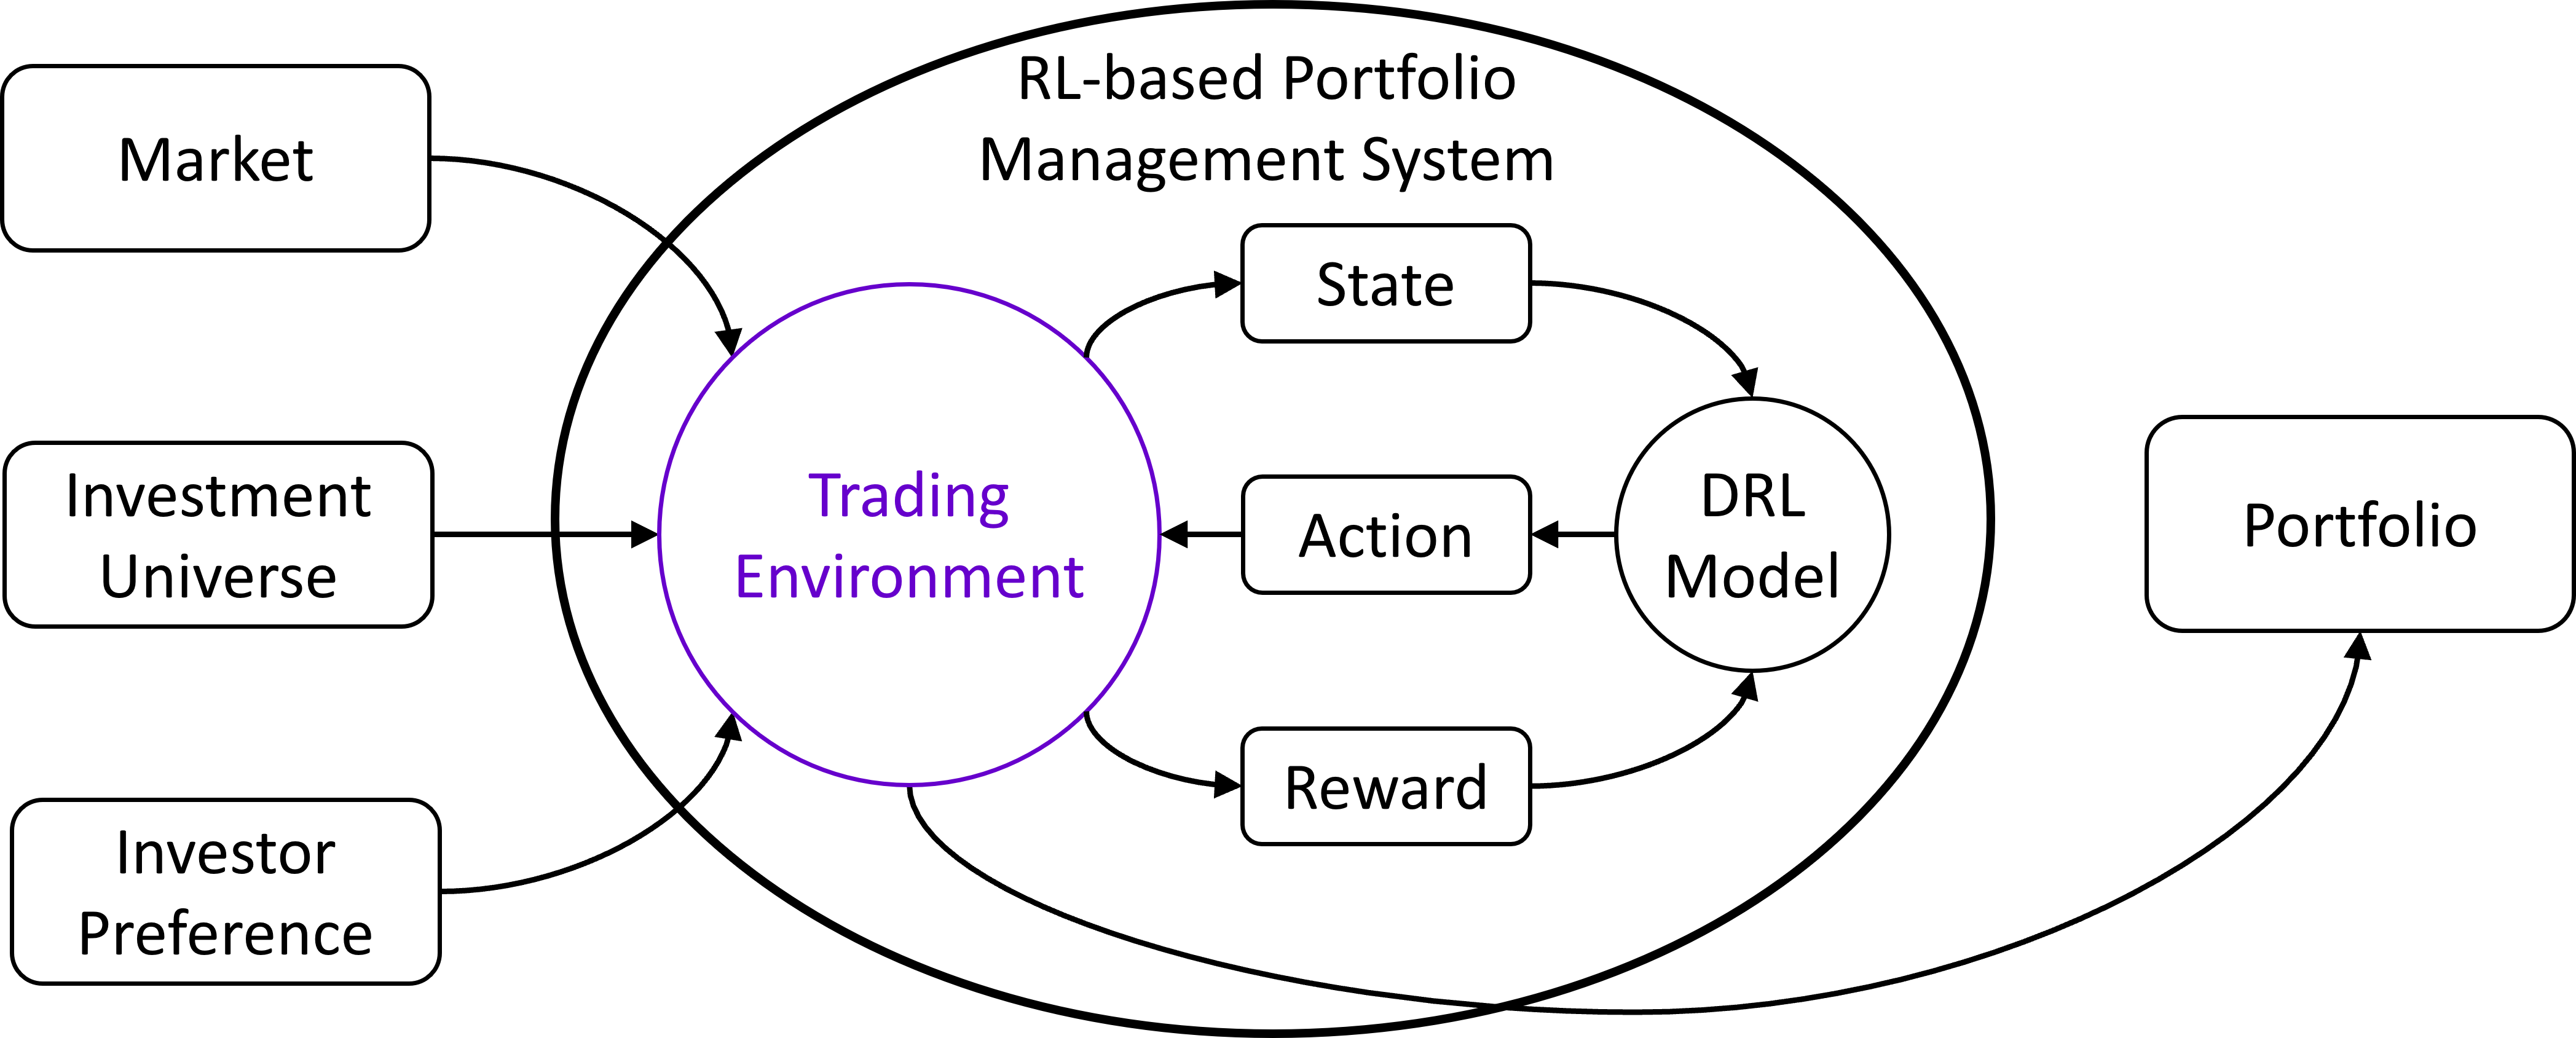
\includegraphics[width=10cm]{images/trading_environment.png}
\end{center}
\end{frame}

\begin{frame}{Feature Extractor}
The feature extractor extracts states from the features.
\begin{enumerate}
    \item {
    Normalize the input features to mean 0 and standard division \(\sigma_{state}\),
        \[
            f^{'}_{i,t} = \frac{\sigma_{state} \times   (f_{i,t} -  \overline{f_i})}{\sigma_{f_i}}
        \]
    }
    \item{To avoid over-fitting, we add Gaussian distribution noise to the feature
            \[
            s_{i,t} = f^{'}_{i,t} + \mathcal{N}(0,\sigma_{noise}^2)
        \]
    }
\end{enumerate}
\alert{Validation results improved significantly after adding noise.}
\begin{center}
  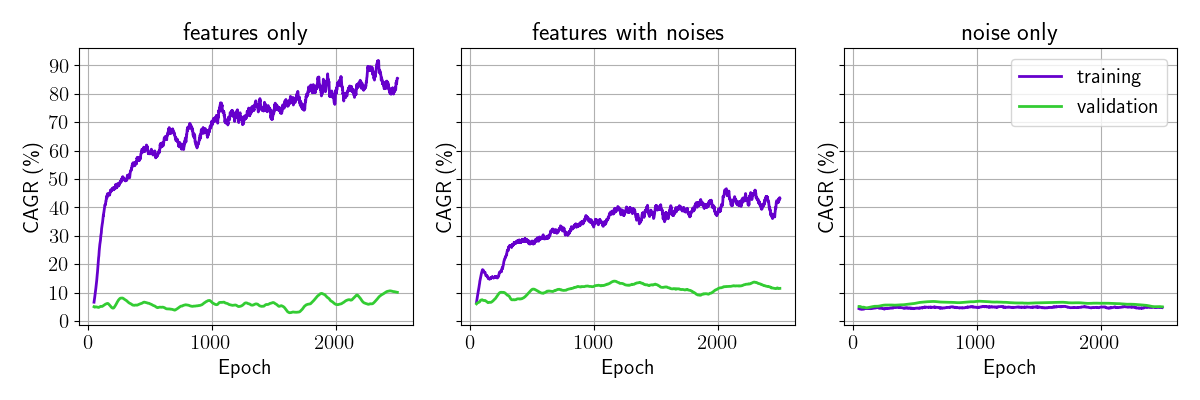
\includegraphics[width=10cm]{images/compare_noise.png}
\end{center}
\end{frame}

\begin{frame}{Portfolio Builder}
The portfolio builder builds the portfolio from the investible universe and the action from the RL model.
\\
\begin{block}{Portfolio}
The portfolio F is an m dimension vector space of weights f.
\[
    F = \{ {f \in \mathbb{R} } \} ^m,
    \sum_{i=1}^m {f_i} =1
\]
\end{block}
\begin{block}{Weight}
Weight is a real number between 0 and 1. \alert{(No short position)}
\[
    f \in \mathbb{R} | 0 \leq f \leq 1 
\]
\end{block}
\end{frame}


\begin{frame}{Trading System}
The Trading System measures performances of the given portfolios
\begin{block}{Performances}
\begin{itemize}
    \item MDD
    \item CAGR
    \item Profit
    \item Wealth
\end{itemize}
\end{block}
These performances will be the input to calculate the reward or evaluate the performance of the system. 
\end{frame}


\begin{frame}{Reward Provider}
The Reward Provider provides the reward to the RL model based on the performance of the portfolio.
\begin{block}{Option 1: Penalty upon negative profits}
Penalty \(p_t-\theta\), upon negative profits exceeding the threshold \(\theta\). 
\[
p_t = \frac{w_t-w_{t-1}}{w_{t-1}}
, 
R_t = 
\begin{cases}
    p_t,&\text{if  }p_t > -\theta\\
    2p_t - \theta ,&\text{if  }p_t \leq  \theta
\end{cases}
\]
\end{block}
\alert{
The result shows unstable improvement in MDD. We observed that the optimization goes too well during training and generates a tiny amount of negative profits; therefore, these negative profits have minimal penalty effect on the model parameters.
}

\end{frame}

\begin{frame}{Reward Provider}
We then apply the penalty upon both positive and negative profits. 
\begin{block}{Option 2: Penalty upon both positive and negative profits}
\[
R_t = 
\begin{cases}
    2p_t - \theta,&\text{if  }    $$|p_t|$$ > \theta\\
    p_t - \theta ,&\text{if  } $$|p_t|$$\leq  \theta
\end{cases}
\]
\end{block}
\alert{This increases the stability significantly.}
\end{frame}



\begin{frame}{Reward Provider}
\begin{columns}
\begin{column}{0.35\textwidth}
The results show penalty upon all profits exceed threshold has much better stability in terms of MDD during validation period. 

\end{column}
\begin{column}{0.65\textwidth}
\begin{center}
      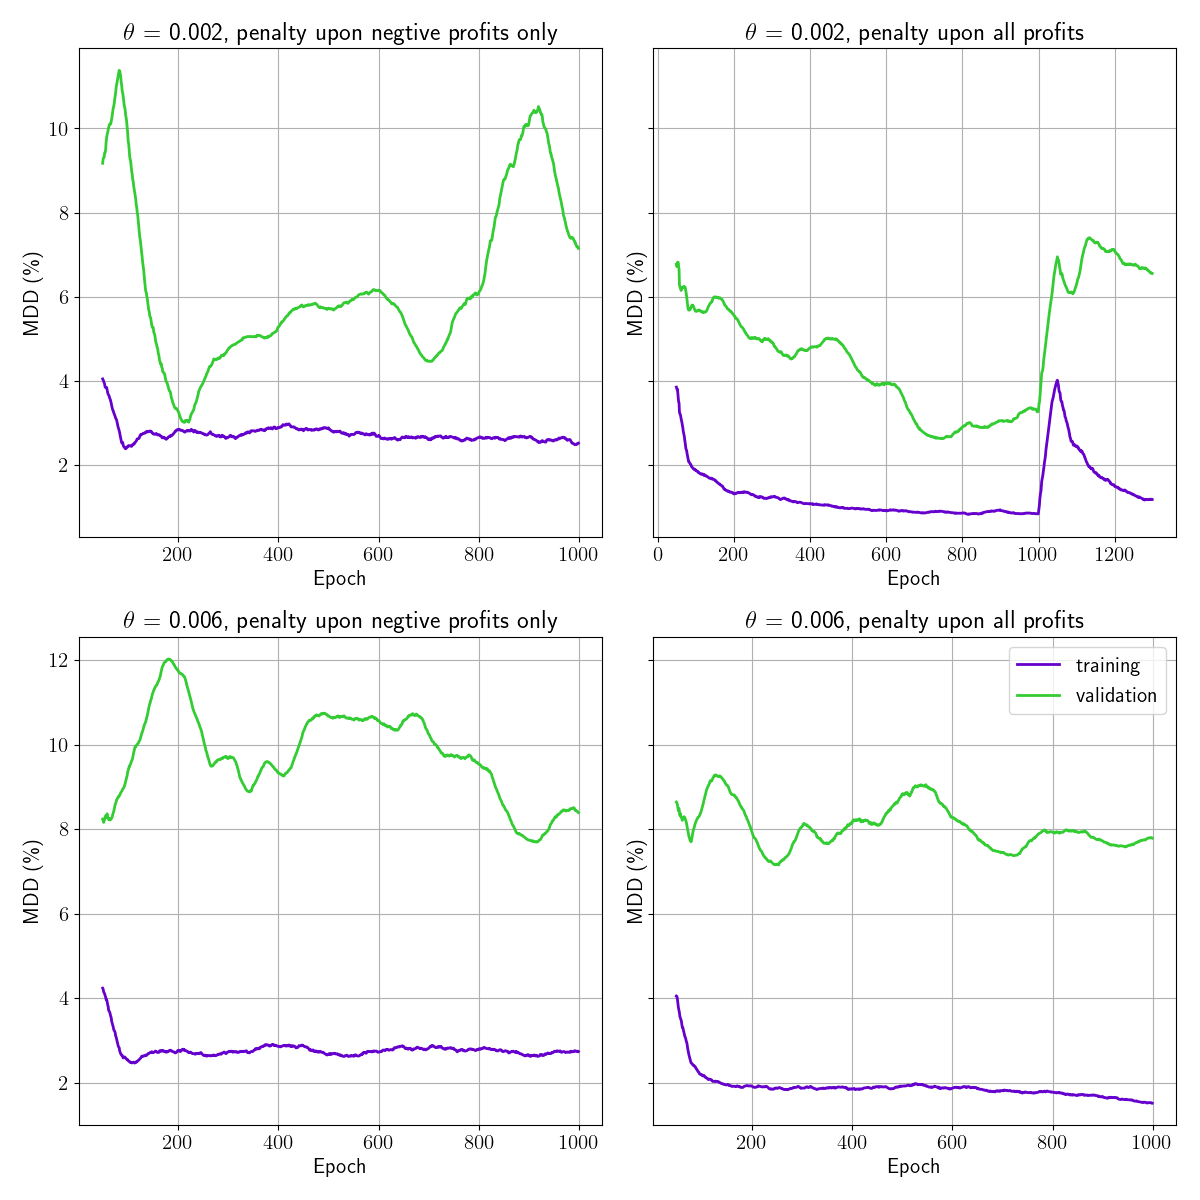
\includegraphics[height=7cm]{images/penalty_negtive_profits_compare.png}
\end{center}
\end{column}
\end{columns}
\end{frame}


\begin{frame}{Validation Result}

\begin{columns}[t]
\begin{column}{0.5\textwidth}
\begin{block}{Validation Period}
Period 1 (2017-03~2019-02) 
\\
Period 2 (2019/03~2021/02)
\end{block}
\begin{block}{Comparison}
Compare CAGR and MDD of the portfolio from our system with result of Constant Rebalanced Portfolio (CRP)
\end{block}
\end{column}

\begin{column}{0.5\textwidth}
\begin{block}{Result}
Our system successfully build portfolios with different MDD upon the same validation period using various thresholds and outperformed CRP Portfolios in most cases.
\end{block}
\end{column}
\end{columns}
\end{frame}

\begin{frame}{Validation Result}
\begin{center}
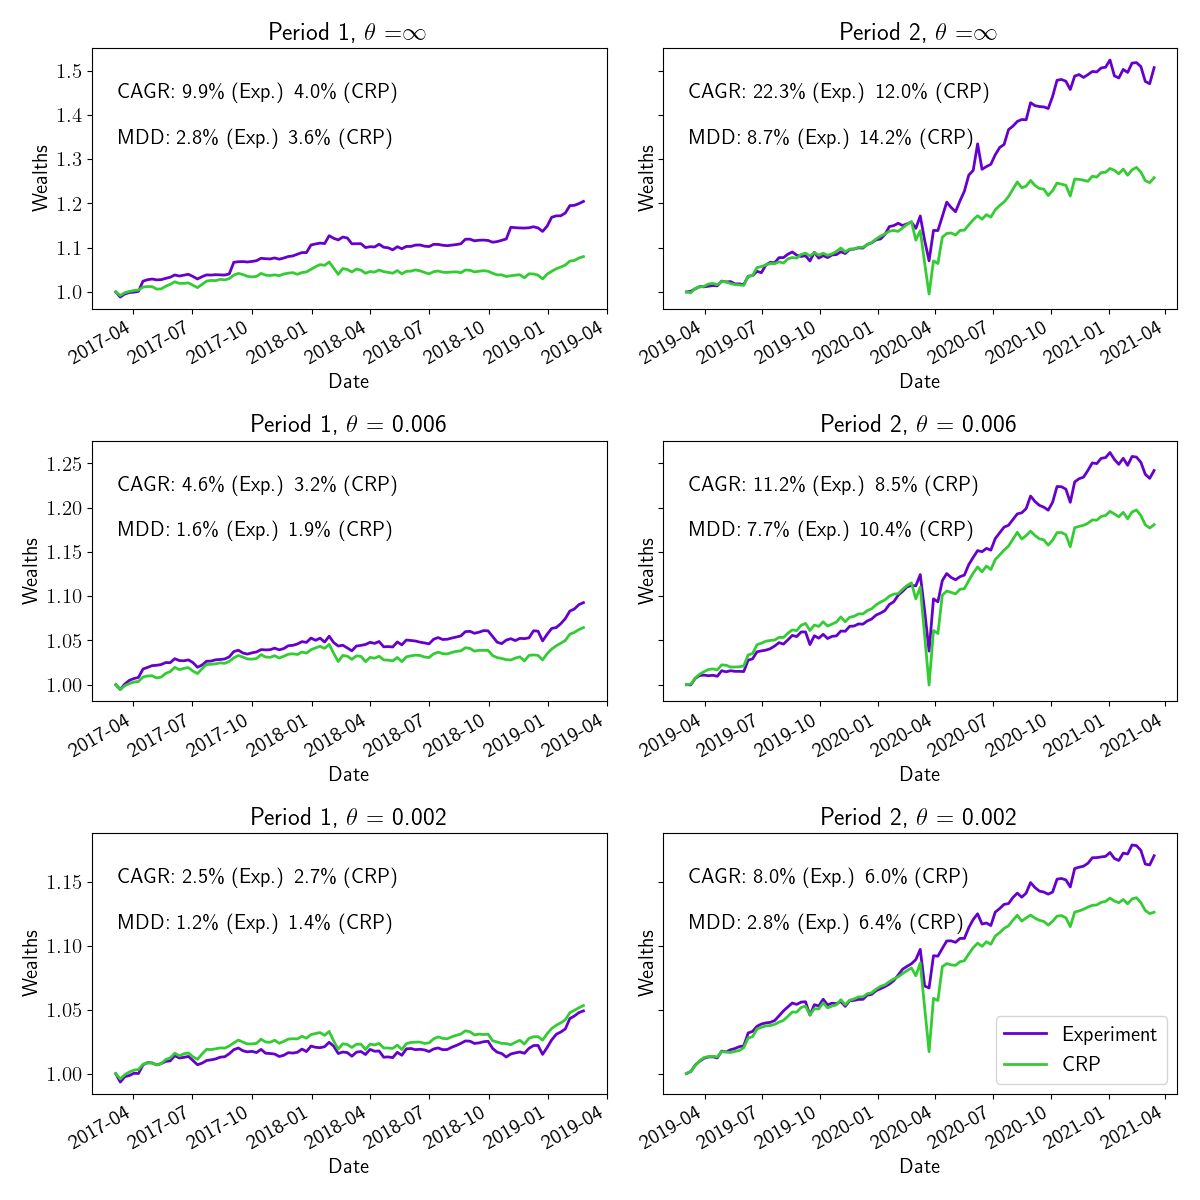
\includegraphics[height= 7.5cm]{images/crp_compare.png}
\end{center}

\end{frame}